\documentclass[12pt]{article}
\usepackage{amsmath}
\usepackage{graphicx}
\usepackage{hyperref}
\usepackage{listings}
\usepackage{color}
\usepackage{pythonhighlight}

\title{Operating System Course Report - First Half of the Semester}
\author{A class}
\date{\today}

\begin{document}

\maketitle
\newpage

\tableofcontents
\newpage

\section{Introduction}
This report summarizes the topics covered during the first half of the Operating System course. It includes theoretical concepts, practical implementations, and assignments. The course focuses on the fundamentals of operating systems, including system architecture, process management, CPU scheduling, and deadlock handling.

\section{Course Overview}
\subsection{Objectives}
The main objectives of this course are:
\begin{itemize}
    \item To understand the basic components and architecture of a computer system.
    \item To learn process management, scheduling, and inter-process communication.
    \item To explore file systems, input/output management, and virtualization.
    \item To study the prevention and handling of deadlocks in operating systems.
\end{itemize}

\subsection{Course Structure}
The course is divided into two halves. This report focuses on the first half, which covers:
\begin{itemize}
    \item Basic Concepts and Components of Computer Systems
    \item System Performance and Metrics
    \item System Architecture of Computer Systems
    \item Process Description and Control
    \item Scheduling Algorithms
    \item Process Creation and Termination
    \item Introduction to Threads
    \item File Systems
    \item Input and Output Management
    \item Deadlock Introduction and Prevention
    \item User Interface Management
    \item Virtualization in Operating Systems
\end{itemize}

\section{Topics Covered}

\subsection{Basic Concepts and Components of Computer Systems}
This section explains the fundamental components that make up a computer system, including the CPU, memory, storage, and input/output devices.

\subsection{System Performance and Metrics}
This section introduces various system performance metrics used to measure the efficiency of a computer system, including throughput, response time, and utilization.

\subsection{System Architecture of Computer Systems}
Describes the architecture of modern computer systems, focusing on the interaction between hardware and the operating system.

\subsection{Process Description and Control}
Processes are a central concept in operating systems. This section covers:
\begin{itemize}
    \item Process states and state transitions
    \item Process control block (PCB)
    \item Context switching
\end{itemize}

\subsubsection{Process Creation}
\textit{Process creation} adalah tahap di mana sistem operasi menciptakan proses baru:
\begin{enumerate}
    \item \textbf{Inisialisasi PCB:} OS membuat \textit{Process Control Block} (PCB) yang berisi informasi dasar proses, seperti Process ID (PID), status awal, dan program \textit{counter}.
    \item \textbf{Masuk ke \textit{Ready Queue}:} Proses ditempatkan dalam \textit{Ready Queue}, menunggu giliran untuk dijadwalkan dan dieksekusi oleh CPU.
    \item \textbf{Alokasi sumber daya:} OS mengalokasikan sumber daya yang diperlukan oleh proses, seperti memori untuk kode dan data, serta akses ke perangkat I/O.
\end{enumerate}

\subsubsection{Process Scheduling}
\textit{Process Scheduling} adalah mekanisme yang berjalan secara terus-menerus untuk menentukan proses mana yang akan dijalankan pada CPU. Penjadwalan terjadi ketika sistem memutuskan proses yang siap untuk dieksekusi atau melakukan \textit{context switching} antara beberapa proses. Tanpa penjadwalan yang baik, sistem tidak bisa mengalokasikan waktu CPU dengan efisien untuk berbagai proses yang ada.

\subsubsection{Process Termination}
\textit{Process Termination} hanya terjadi ketika proses tersebut sudah tidak diperlukan lagi, entah karena telah selesai dieksekusi, terjadi kesalahan, atau karena dihentikan oleh pengguna atau OS. Proses yang dihentikan akan dibuang dari sistem (PCB dihapus, memori dibebaskan), dan tidak lagi dijadwalkan untuk berjalan.

\subsubsection{Context Switching}
\textit{Context switching} adalah mekanisme yang memungkinkan sistem operasi untuk berpindah dari satu proses ke proses lain. Setiap kali terjadi perpindahan, OS perlu menyimpan \textit{state} dari proses yang sedang berjalan (misalnya nilai \textit{register}, program \textit{counter , stack pointer,} dll.) dan memuat \textit{state} dari proses yang akan dijalankan. Proses penyimpanan dan pemuatan ini memerlukan waktu dan sumber daya, sehingga \textit{context switching} dianggap sebagai \textit{overhead} dalam sistem multitasking. Dalam sistem \textit{preemptive multitasking}, di mana proses-proses dihentikan secara paksa oleh OS untuk memberikan giliran pada proses lain, \textit{}context switching menjadi sangat penting untuk menjaga ilusi bahwa semua proses berjalan secara bersamaan. Proses ini terjadi ketika CPU berpindah dari satu proses ke proses lain, atau dari proses ke kernel mode, misalnya saat menangani \textit{interrupts}.



\subsection{Scheduling Algorithms}
This section covers:
\begin{itemize}
    \item First-Come, First-Served (FCFS)
    \item Shortest Job Next (SJN)
    \item Round Robin (RR)
\end{itemize}
It explains how these algorithms are used to allocate CPU time to processes.

\subsection{Process Creation and Termination}
Details how processes are created and terminated by the operating system, including:
\begin{itemize}
    \item Process spawning
    \item Process termination conditions
\end{itemize}

\subsection{Introduction to Threads}
This section introduces the concept of threads and their relation to processes, covering:
\begin{itemize}
    \item Single-threaded vs. multi-threaded processes
    \item Benefits of multithreading
\end{itemize}

\begin{figure}[h]
    \centering
    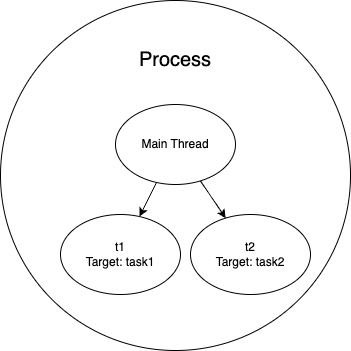
\includegraphics[width=0.5\textwidth]{/Users/khawaritzmi/Unhas/os_report_mid2024/a_class/asset/example.png}  % Sesuaikan nama file dan ukurannya
    \caption{Ini adalah gambar contoh dari multithreading.}
    \label{fig:contoh_gambar}
\end{figure}

Seperti yang terlihat pada Gambar \ref{fig:contoh_gambar}, inilah cara menambahkan gambar dengan keterangan.

\subsection{File Systems}
File systems provide a way for the operating system to store, retrieve, and manage data. This section explains:
\begin{itemize}
    \item File system structure
    \item File access methods
    \item Directory management
\end{itemize}

\subsection{Input and Output Management}
Input and output management is key for handling the interaction between the system and external devices. This section includes:
\begin{itemize}
    \item Device drivers
    \item I/O scheduling
\end{itemize}

\subsection{Deadlock Introduction and Prevention}
Explores the concept of deadlocks and methods for preventing them:
\begin{itemize}
    \item Deadlock conditions
    \item Deadlock prevention techniques
\end{itemize}

\subsection{User Interface Management}
This section discusses the role of the operating system in managing the user interface. Topics covered include:
\begin{itemize}
    \item Graphical User Interface (GUI)
    \item Command-Line Interface (CLI)
    \item Interaction between the user and the operating system
\end{itemize}

\subsection{Virtualization in Operating Systems}
Virtualization allows multiple operating systems to run concurrently on a single physical machine. This section explores:
\begin{itemize}
    \item Concept of virtualization
    \item Hypervisors and their types
    \item Benefits of virtualization in modern computing
\end{itemize}

\section{Assignments and Practical Work}
\subsection{Assignment 1: Process Scheduling}
Students were tasked with implementing various process scheduling algorithms (e.g., FCFS, SJN, and RR) and comparing their performance under different conditions.
\subsubsection{Group 1}
\begin{python}
    class Process:
    def __init__(self, pid, arrival_time, burst_time):
        self.pid = pid
        self.arrival_time = arrival_time
        self.burst_time = burst_time
        self.completion_time = 0
        self.turnaround_time = 0
        self.waiting_time = 0
\end{python}

\begin{table}[htbp] % Optional: For floating position
    \centering
    \begin{tabular}{|c|c|c|} % Defines number of columns and alignment (c = center, l = left, r = right). '|' creates vertical lines.
    \hline
    Header 1 & Header 2 & Header 3 \\ % Column headers
    \hline
    Row 1, Column 1 & Row 1, Column 2 & Row 1, Column 3 \\ % First row of data
    \hline
    Row 2, Column 1 & Row 2, Column 2 & Row 2, Column 3 \\ % Second row of data
    \hline
    \end{tabular}
    \caption{Your table caption} % Optional: For adding a caption
    \label{tab:your_label} % Optional: For cross-referencing the table
\end{table}
\subsection{Assignment 2: Deadlock Handling}
In this assignment, students were asked to simulate different deadlock scenarios and explore various prevention methods.

\subsection{Assignment 3: Multithreading and Amdahl's Law}
This assignment involved designing a multithreading scenario to solve a computationally intensive problem. Students then applied **Amdahl's Law** to calculate the theoretical speedup of the program as the number of threads increased.

\subsection{Assignment 4: Simple Command-Line Interface (CLI) for User Interface Management}
Students were tasked with creating a simple **CLI** for user interface management. The CLI should support basic commands such as file manipulation (creating, listing, and deleting files), process management, and system status reporting.

\subsection{Assignment 5: File System Access}
In this assignment, students implemented file system access routines, including:
\begin{itemize}
   \item \textbf{File creation and deletion}: \textit{File creation} adalah proses menciptakan berkas baru dalam sistem berkas. Ini dilakukan dengan mendefinisikan nama berkas dan format yang diinginkan, lalu menyimpan data ke dalam berkas tersebut. Contohnya, saat kita membuat berkas teks, kita dapat menyimpan berbagai informasi atau data di dalamnya.
    
    Sebaliknya, \textit{deletion} adalah proses menghilangkan berkas yang sudah ada dan tidak lagi diperlukan. Hal ini penting untuk mengelola ruang penyimpanan serta menjaga sistem tetap rapi. Saat menghapus berkas, kita perlu memastikan bahwa berkas yang akan dihapus benar-benar ada, agar tidak terjadi kesalahan.
    
    \item \textbf{Reading from and writing to files}: \textit{Reading} berarti mengambil data yang tersimpan dalam berkas untuk digunakan dalam program atau ditampilkan kepada pengguna. Proses ini memungkinkan kita memanfaatkan informasi yang telah ada tanpa harus membuatnya ulang. Misalnya, kita bisa membaca daftar nama dari sebuah berkas dan menampilkannya di layar.
    
    \textit{Writing} adalah proses menyimpan data ke dalam berkas. Ini dapat dilakukan dengan menambahkan informasi baru ke berkas yang sudah ada atau membuat berkas baru jika belum ada. Proses ini sangat berguna untuk menyimpan hasil kerja, catatan, atau informasi penting lainnya agar dapat diakses di lain waktu.
    
    \item \textbf{Navigating directories and managing file permissions}: \textit{Navigating directories} adalah kemampuan untuk berpindah antara berbagai folder atau direktori dalam sistem berkas. Ini penting karena berkas dan direktori biasanya disusun dalam hirarki, sehingga kita perlu dapat menavigasi struktur tersebut untuk menemukan berkas yang dibutuhkan.
    
    \textit{Managing file permissions} adalah proses mengatur siapa yang dapat mengakses dan memodifikasi berkas tertentu. Dalam sistem operasi, izin dapat ditetapkan untuk pengguna tertentu, kelompok, atau semua orang. Hal ini membantu menjaga keamanan data dan memastikan bahwa hanya orang yang berwenang yang dapat mengubah atau menghapus berkas. Misalnya, izin baca, tulis, dan eksekusi dapat diatur untuk setiap berkas dan direktori, memberikan kontrol penuh terhadap akses data.

    \item \textbf{Contoh soal dan pengimplementasian pada code python}:
    Buatlah program Python yang melakukan hal berikut:
    Membuat berkas bernama data.txt, menulis tiga kalimat ke dalam berkas tersebut. membaca isi berkas dan menampilkannya di layar, menghapus berkas data.txt.

    \begin{python}
    def create_and_write_file(filename, content):
    try:
        with open(filename, 'w') as file:
            file.write(content)
        print(f"Berkas '{filename}' telah dibuat dan ditulis.")
    except Exception as e:
        print(f"Terjadi kesalahan saat membuat atau menulis berkas: {e}")

# 2. Membaca isi berkas
def read_file(filename):
    try:
        if os.path.exists(filename):
            with open(filename, 'r') as file:
                content = file.read()
                print(f"Isi berkas '{filename}':\n{content}")
        else:
            print(f"Berkas '{filename}' tidak ditemukan.")
    except Exception as e:
        print(f"Terjadi kesalahan saat membaca berkas: {e}")

# 3. Menghapus berkas
def delete_file(filename):
    try:
        if os.path.exists(filename):
            os.remove(filename)
            print(f"Berkas '{filename}' telah dihapus.")
        else:
            print(f"Berkas '{filename}' tidak ditemukan.")
    except Exception as e:
        print(f"Terjadi kesalahan saat menghapus berkas: {e}")
        # Implementasi
filename = input("Masukkan nama berkas (misalnya 'data.txt'): ")
content = input("Masukkan konten yang ingin ditulis ke dalam berkas:\n")

create_and_write_file(filename, content)  # Membuat dan menulis berkas
read_file(filename)                        # Membaca isi berkas
delete_file(filename)                      # Menghapus berkas

    \end{python}
    \item \textb{Output}: Saat menjalankan program, output yang dihasilkan akan seperti berikut:
\begin{verbatim}
Masukkan nama berkas (misalnya 'data.txt'): data.txt
Masukkan konten yang ingin ditulis ke dalam berkas:
Ini adalah kalimat pertama.
Ini adalah kalimat kedua.
Ini adalah kalimat ketiga.
Berkas 'data.txt' telah dibuat dan ditulis.
Isi berkas 'data.txt':
Ini adalah kalimat pertama.
Ini adalah kalimat kedua.
Ini adalah kalimat ketiga.
Berkas 'data.txt' telah dihapus.
\end{verbatim}
\end{python}
\end{itemize}

\section{Conclusion}
The first half of the course introduced core operating system concepts, including process management, scheduling, multithreading, and file system access. These topics provided a foundation for more advanced topics to be covered in the second half of the course.

\end{document}